\documentclass[ucs,9pt]{beamer}

% Copyright 2004 by Till Tantau <tantau@users.sourceforge.net>.
%
% In principle, this file can be redistributed and/or modified under
% the terms of the GNU Public License, version 2.
%
% However, this file is supposed to be a template to be modified
% for your own needs. For this reason, if you use this file as a
% template and not specifically distribute it as part of a another
% package/program, I grant the extra permission to freely copy and
% modify this file as you see fit and even to delete this copyright
% notice.
%
% Modified by Tobias G. Pfeiffer <tobias.pfeiffer@math.fu-berlin.de>
% to show usage of some features specific to the FU Berlin template.

% remove this line and the "ucs" option to the documentclass when your editor is not utf8-capable
\usepackage[utf8x]{inputenc}    % to make utf-8 input possible
\usepackage[english,german]{babel}     % hyphenation etc., alternatively use 'german' as parameter

% Template for talks using the Corporate Design of the Freie Universitaet
%   Berlin, created following the guidelines on www.fu-berlin.de/cd by
%   Tobias G. Pfeiffer, <tobias.pfeiffer@math.fu-berlin.de>
% This file can be redistributed and/or modified in any way you like.
%   If you feel you have done significant improvements to this template,
%   please consider providing your modified version to
%   https://www.mi.fu-berlin.de/w/Mi/BeamerTemplateCorporateDesign

\usepackage{amsmath,dsfont,listings}

%%% FU logo
% small version for upper right corner of normal pages
\pgfdeclareimage[height=0.9cm]{university-logo}{FULogo_RGB}
\logo{\pgfuseimage{university-logo}}
% large version for upper right corner of title page
\pgfdeclareimage[height=1.085cm]{big-university-logo}{FULogo_RGB}
\newcommand{\titleimage}[1]{\pgfdeclareimage[height=2.92cm]{title-image}{#1}}
\titlegraphic{\pgfuseimage{title-image}}
%%% end FU logo

% NOTE: 1cm = 0.393 in = 28.346 pt;    1 pt = 1/72 in = 0.0352 cm
\setbeamersize{text margin right=3.5mm, text margin left=7.5mm}  % text margin

% colors to be used
\definecolor{text-grey}{rgb}{0.45, 0.45, 0.45} % grey text on white background
\definecolor{bg-grey}{rgb}{0.66, 0.65, 0.60} % grey background (for white text)
\definecolor{fu-blue}{RGB}{0, 51, 102} % blue text
\definecolor{fu-green}{RGB}{153, 204, 0} % green text
\definecolor{fu-red}{RGB}{204, 0, 0} % red text (used by \alert)

% switch off the sidebars
% TODO: loading \useoutertheme{sidebar} (which is maybe wanted) also inserts
%   a sidebar on title page (unwanted), also indents the page title (unwanted?),
%   and duplicates the navigation symbols (unwanted)
\setbeamersize{sidebar width left=0cm, sidebar width right=0mm}
\setbeamertemplate{sidebar right}{}
\setbeamertemplate{sidebar left}{}
%    XOR
% \useoutertheme{sidebar}

% frame title
% is truncated before logo and splits on two lines
% if neccessary (or manually using \\)
\setbeamertemplate{frametitle}{%
    \vskip-30pt \color{text-grey}\large%
    \begin{minipage}[b][23pt]{80.5mm}%
    \flushleft\insertframetitle%
    \end{minipage}%
}

%%% title page
% TODO: get rid of the navigation symbols on the title page.
%   actually, \frame[plain] *should* remove them...
\setbeamertemplate{title page}{
% upper right: FU logo
\vskip2pt\hfill\pgfuseimage{big-university-logo} \\
\vskip6pt\hskip3pt
% title image of the presentation
\begin{minipage}{11.6cm}
\hspace{-1mm}\inserttitlegraphic
\end{minipage}

% set the title and the author
\vskip14pt
\parbox[top][1.35cm][c]{11cm}{\color{text-grey}\inserttitle \\ \small \insertsubtitle}
\vskip11pt
\parbox[top][1.35cm][c]{11cm}{\small \insertauthor \\ \insertinstitute \\[3mm] \insertdate}
}
%%% end title page

%%% colors
\usecolortheme{lily}
\setbeamercolor*{normal text}{fg=black,bg=white}
\setbeamercolor*{alerted text}{fg=fu-red}
\setbeamercolor*{example text}{fg=fu-green}
\setbeamercolor*{structure}{fg=fu-blue}

\setbeamercolor*{block title}{fg=white,bg=black!50}
\setbeamercolor*{block title alerted}{fg=white,bg=black!50}
\setbeamercolor*{block title example}{fg=white,bg=black!50}

\setbeamercolor*{block body}{bg=black!10}
\setbeamercolor*{block body alerted}{bg=black!10}
\setbeamercolor*{block body example}{bg=black!10}

\setbeamercolor{bibliography entry author}{fg=fu-blue}
% TODO: this doesn't work at all:
\setbeamercolor{bibliography entry journal}{fg=text-grey}

\setbeamercolor{item}{fg=fu-blue}
\setbeamercolor{navigation symbols}{fg=text-grey,bg=bg-grey}
%%% end colors

%%% headline
\setbeamertemplate{headline}{
\vskip4pt\hfill\insertlogo\hspace{3.5mm} % logo on the right

\vskip6pt\color{fu-blue}\rule{\textwidth}{0.4pt} % horizontal line
}
%%% end headline

%%% footline
\newcommand{\footlinetext}{\insertshortinstitute, \insertshorttitle, \insertshortdate}
\setbeamertemplate{footline}{
\vskip5pt\color{fu-blue}\rule{\textwidth}{0.4pt}\\ % horizontal line
\vskip2pt
\makebox[123mm]{\hspace{7.5mm}
\color{fu-blue}\footlinetext
\hfill \raisebox{-1pt}{\usebeamertemplate***{navigation symbols}}
\hfill \insertframenumber}
\vskip4pt
}
%%% end footline

%%% settings for listings package
\lstset{extendedchars=true, showstringspaces=false, basicstyle=\footnotesize\sffamily, tabsize=2, breaklines=true, breakindent=10pt, frame=l, columns=fullflexible}
\lstset{language=Java} % this sets the syntax highlighting
\lstset{mathescape=true} % this switches on $...$ substitution in code
% enables UTF-8 in source code:
\lstset{literate={ä}{{\"a}}1 {ö}{{\"o}}1 {ü}{{\"u}}1 {Ä}{{\"A}}1 {Ö}{{\"O}}1 {Ü}{{\"U}}1 {ß}{\ss}1}
%%% end listings  % THIS is the line that includes the FU template!

\usepackage{arev,t1enc} % looks nicer than the standard sans-serif font
% if you experience problems, comment out the line above and change
% the documentclass option "9pt" to "10pt"

% image to be shown on the title page (without file extension, should be pdf or png)
\titleimage{fu_500}

\title{SWP Übersetzerbau im SS 12}
\subtitle{Informationen und Organisatorisches}
\author{Maximilian~Konzack \and Tim~Rakowski}
\institute[FU Berlin]{Freie Universität Berlin}

\date{Einführungsveranstaltung am 12.~April 2012}


% you can redefine the text shown in the footline. use a combination of
% \insertshortauthor, \insertshortinstitute, \insertshorttitle, \insertshortdate, ...
\renewcommand{\footlinetext}{\insertshortinstitute, \insertshorttitle, \insertshortdate}

% Delete this, if you do not want the table of contents to pop up at
% the beginning of each subsection:
%\AtBeginSubsection[]
%{
%  \begin{frame}<beamer>{Outline}
%    \tableofcontents[currentsection,currentsubsection]
%  \end{frame}
%}

\begin{document}

\begin{frame}[plain]
  \titlepage
\end{frame}

\begin{frame}{Übersicht}
  \tableofcontents
\end{frame}

\section{Projektidee}
\begin{frame}
  \frametitle{Entwicklung eines Compilers im Team}
  \begin{center}
    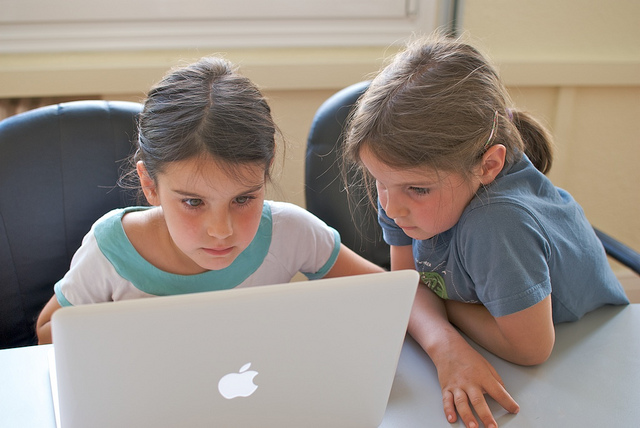
\includegraphics[width=0.7\textwidth]{pair_prog}
  \end{center}
\end{frame}
\begin{frame}
  \frametitle{Modularer Compiler}
  \begin{block}{Idee}
    \begin{itemize}
      \item Arbeit an einem Übersetzer
      \item viele kleine Teilprojekte für Compilerkette
      \item Quellsprache ist imperativ und statisch typisiert
      \item Zwischencode kann von anderen Compilern genutzt werden
    \end{itemize}
  \end{block}

  \begin{columns}
    \begin{column}{0.3\textwidth}
  \begin{center}
    
\includegraphics[height=3cm]{java_duke}
  \end{center}
\end{column}
    \begin{column}{0.7\textwidth}
  \begin{block}{Ziele}
    \begin{enumerate}
      \item Kommunikation zwischen den Teilprojekten!
      \item Modulare Komponenten für die Teilprojekte
      \item LLVM als Zwischencode
      \item Absprache von Schnittstellen
      \item Implementierungssprache ist Java
    \end{enumerate}
  \end{block}
\end{column}
  \end{columns}
\end{frame}

\section{Vorstellung der Projekte}
\subsection{Händisch erstellter Frontend}
\begin{frame}
  \frametitle{Händische Entwicklung eines Übersetzers}

  \begin{block}{Aufgaben}
    \begin{enumerate}
      \item Softwaredesign und -architektur für das Projekt
      \item Implementierung eines Lexers, Parsers mit Codegenerierung mittels einfacher Übersetzerbautechniken
      \item Verwaltung der Interfaces alle Phasen und ihrer Kontrolle (z.B. Token, Symboltabelle, abstrakter Syntaxbaum, \ldots) 
    \end{enumerate}
  \end{block}

  \begin{block}{Gruppengröße}
    6 bis 8 Personen
  \end{block}
\end{frame}

\subsection{Lexergenerator}
\begin{frame}
  \frametitle{Entwicklung eines Lexergenerators}

  \begin{block}{Aufgaben}
    \begin{enumerate}
      \item Erzeugung eines funktionsfähigen Lexers
      \item Eingabe für den Generator sind reguläre Definitionen
      \item Tokenerkennung soll über endliche Automaten erfolgen 
    \end{enumerate}
  \end{block}

  \begin{block}{Gruppengröße}
    2 bis 4 Personen
  \end{block}
\end{frame}

\subsection{Parsergenerator}
\begin{frame}
  \frametitle{Entwicklung eines Parsergenerators}

  \begin{block}{Aufgaben}
    \begin{enumerate}
      \item Erzeugung eines tabellengetriebenen LL(1)-Parsers
      \item Eingabe für den Generator ist eine Grammatikdefinition in BNF
      \item Erstellung eines konkreten Syntaxbaums (Parsebaums) zur weiteren Verarbeitung in
        Folgephasen
    \end{enumerate}
  \end{block}

  \begin{block}{Gruppengröße}
    2 bis 4 Personen
  \end{block}
\end{frame}

\subsection{Semantische Analyse}
\begin{frame}
  \frametitle{Durchführung von semantischen Analysen}

  \begin{block}{Aufgaben}
    \begin{enumerate}
      \item Alle Analysen dekorieren oder modifizieren den abstrakten Syntaxbaum
        \begin{itemize}
          \item Typüberprüfung und -inferenz
          \item Erzeugung aussagekräftiger Fehlermeldungen
          \item Zwischencodegenerierung
          \item Intrumentierung des Zwischencodes
        \end{itemize}
          \item Ausgabe ist LLVM-Zwischencode 
    \end{enumerate}
  \end{block}

  \begin{block}{Gruppengröße}
    2 bis 4 Personen
  \end{block}
\end{frame}

\subsection{Optimierungstechniken}
\begin{frame}
  \frametitle{Anwendung von Optimierungstechniken}

  \begin{block}{Aufgaben}
    \begin{enumerate}
        \item Eingabe ist LLVM-Zwischencode
        \item Ausgabe erfolgt als optimierter LLVM-Zwischencode
        \item Teilaufgaben sind
          \begin{itemize}
            \item Gemeinsame Teilausdrücke
            \item Eliminierung von totem (unerreichbarem) Code
            \item def-use-Ketten: Warning bei deklarierten, aber nicht verwendeten Variablen
            \item weitere Datenflussanalysen 
          \end{itemize}
    \end{enumerate}
  \end{block}

  \begin{block}{Gruppengröße}
    2 bis 4 Personen
  \end{block}
\end{frame}

\subsection{Maschinencodegenerierung}
\begin{frame}
  \frametitle{Generierung von Maschinencode}

  \begin{block}{Aufgaben}
    \begin{enumerate}
      \item Eingabe ist LLVM-Zwischencode
      \item Ausgabe erfolgt als ausführbarer Maschinencode
      \item z.B. Java Byte Code, Intel Assembler, GNU AS, \ldots 
    \end{enumerate}
  \end{block}

  \begin{block}{Gruppengröße}
    2 bis 4 Personen
  \end{block}
\end{frame}


\section{Infrastruktur des Projekts}
\subsection{Low Level Virtual Machine}
\begin{frame}
  \frametitle{Was ist die Low Level Virtual Machine (LLVM)?}
  \begin{columns}
    \begin{column}{0.3\textwidth}
      \begin{center}
        
\includegraphics[width=3cm]{llvm_logo}
      \end{center}
    \end{column}
    \begin{column}{0.7\textwidth}
      \begin{block}{Ziele}
        \begin{itemize}
          \item Unterstützung vielfältiger Compilertechniken
          \item stabiler Intermediate Code
          \item anpassbar für verschiedene Aufgaben
        \end{itemize}
      \end{block}
      \begin{block}{Aufgaben}
        \begin{itemize}
          \item verschieden Quellsprachen
          \item Zwischencodeerzeugung
          \item Optimierungen
          \item Debugging
          \item Statische Analysen
          \item \dots
        \end{itemize}
      \end{block}
    \end{column}
  \end{columns}
\end{frame}

\begin{frame}[fragile]
  \frametitle{Beispiel in C}
  \begin{verbatim}
int adder(int a, int b)
  {
    int c = a + b;
    return c;
  }


int main(void) {
  int sum = adder(5,7);
  printf("sum = %i\n",sum);
  printf("hello world\n");
  return 0;
}
  \end{verbatim}
\end{frame}

\begin{frame}[fragile]
  \frametitle{LLVM Zwischencode}
  \begin{verbatim}
@.str = private constant [10 x i8] c"sum = %i\0A\00"
@.str1 = private constant [13 x i8] c"hello world\0A\00"

define i32 @adder(i32 %a, i32 %b) nounwind {
  %1 = alloca i32, align 4
  %2 = alloca i32, align 4
  %c = alloca i32, align 4
  store i32 %a, i32* %1, align 4
  store i32 %b, i32* %2, align 4
  %3 = load i32* %1, align 4
  %4 = load i32* %2, align 4
  %5 = add nsw i32 %3, %4
  store i32 %5, i32* %c, align 4
  %6 = load i32* %c, align 4
  ret i32 %6
}
  \end{verbatim}
\end{frame}

\begin{frame}[fragile]
  \frametitle{Umsetzung der \texttt{main()}-Funktion}
  \begin{verbatim}
define i32 @main() nounwind {
  %1 = alloca i32, align 4
  %sum = alloca i32, align 4
  store i32 0, i32* %1
  %2 = call i32 @adder(i32 5, i32 7)
  store i32 %2, i32* %sum, align 4
  %3 = load i32* %sum, align 4
  %4 = call i32 (i8*, ...)* @printf(i8* getelementptr inbounds ([10 x i8]* @.str, i32 0, i32 0), i32 %3)
  %5 = call i32 (i8*, ...)* @printf(i8* getelementptr inbounds ([13 x i8]* @.str1, i32 0, i32 0))
  ret i32 0
}

declare i32 @printf(i8*, ...)
  \end{verbatim}
\end{frame}

\subsection{Repository}
\begin{frame}
  \frametitle{Wie soll das Projekt verwaltet werden?}
  \begin{center}
    \Huge Subversion vs. Git
  \end{center}
\end{frame}

\section{Organisatorisches}
\subsection{Treffen}
\begin{frame}
  \frametitle{Projekttreffen}
  \begin{block}{Treffen aller Teilnehmer}
    \begin{itemize}
      \item wöchentlich
      \item donnerstags von 10 bis 12 Uhr c.t.
      \item jedes Team berichtet ca. 5~Min. über Status, Probleme, \dots
      \item anschließend kurze Diskussion möglich (5 bis 10 Min.)
      \item bei zu vielen Fehlterminen wird Anwesenheitspflicht eingeführt!
    \end{itemize}
  \end{block}

  \begin{block}{Projekttreffen}
    \begin{enumerate}
      \item interne Treffen eigenständig organisieren
      \item regelmäßige Treffen mit Tim, Max und bei Bedarf andere Teams
      \item Ansprechpartner für SWP Betreuer festlegen!
      \item Agenda für Treffen vorbereiten oder besser an uns schicken
    \end{enumerate}
  \end{block}
\end{frame}

\subsection{Zuteilung der Projekte}
\begin{frame}
  \frametitle{Zuteilung der Projekte}
  \begin{enumerate}
    \item Verteilen der Listen
    \item Maximal 2x Eintragen
    \item Wünsche bitte über Anmerkung notieren
    \item Zuteilung erfolgt heute!
  \end{enumerate}
\end{frame}

\section{Ende}
\begin{frame}
  \frametitle{Ende}
  \begin{center}
    \Huge
    Danke für die Aufmerksamkeit.\\[1em]
    
\includegraphics[height=5cm]{compilers}
    \ 
  \end{center}
\end{frame}

\begin{frame}
  \frametitle{Weiteres Vorgehen}
  \begin{enumerate}
    \item Gruppeneinfindung
      \begin{itemize}
        \item interne Treffen organisieren
        \item Ansprechpartner für Tim und Max
        \item Erste Konzepte entwerfen: Interfaces, Beispielsyntax, \dots
        \item Probleme festhalten
        \item Absprache mit anderen Teams?
      \end{itemize}
    \item Repository einrichten
    \item Quellsprache verstehen
    \item LLVM näher kennen lernen
    \item Literatur konsultieren
  \end{enumerate}
\end{frame}

% All of the following is optional and typically not needed. 
\appendix
\section*{\appendixname}

\begin{frame}
  \frametitle{Literatur}
    
  \begin{thebibliography}{10}
    
  \beamertemplatebookbibitems
  % Start with overview books.

  
  \bibitem[AUS08]{Aho08}
    Alfred~V. Aho, Jeffrey Ullman, and Ravi Sethi.
    \newblock {\em Compiler: {P}rinzipien, {T}echniken und {W}erkzeuge}.
    \newblock Pearson Studium, 2. edition, 2008.


  \bibitem[Fin]{FindBugsWeb}
    {F}ind{B}ugs -- {F}ind {B}ugs in {J}ava {P}rograms.
    \newblock {\url{http://findbugs.sourceforge.net/}}.


  \bibitem[LA04]{Lattner04}
    Chris Lattner and Vikram~S. Adve.
    \newblock {LLVM}: {A} compilation framework for lifelong program analysis \&
      transformation.
      \newblock In {\em CGO}, pages 75--88. IEEE Computer Society, 2004.

    \bibitem[Lat02]{Lattner00diss}
      Chris~Arthur Lattner.
      \newblock {LLVM}: An infrastructure for multi-stage optimization, 2002.

    \bibitem[Sco09]{Scott09}
      Michael~Lee Scott.
      \newblock {\em Programming language pragmatics}.
      \newblock Morgan Kaufmann Publishers, 3. edition, 2009.
    
  \end{thebibliography}
\end{frame}

\end{document}
